\chapter{Contributions}\label{chap:contributions}

All the work I have done during this internship is related to the \gls{pfw},
which was briefly presented in section \ref{sec:parameter-framework}.

% {{{1
\section{Parameter-framework core enhancements}

% {{{2
\subsection{XML validation at build time}
\subsubsection{Build process}
FIXME FIXME forward reference, this is no good.
The pfw language as described in \ref{desc:pfw-language} is used for rule based
description. Those are translated into \gls{xml} files during the build via a
specific make target.  In order to generate those \gls{xml} files, we also need
the information of the Structure files, which are written by the integration
engineers.

To generate those files, we rely on a toolset we call \emph{HostDomainGenerator}.
The figure \ref{fig:build-process} shows how it works:

\begin{figureGraphics}{Xml generation build process}{fig:build-process}
    \includegraphics[height=0.4\textheight]{./src/img/build-generation.pdf}
\end{figureGraphics}

But there were some limitations. Since the writing of the \gls{xml} structure files is done by human beings, there was
\emph{no guarantee} that their files were semantically correct.
Since no check was done during the build-process, the generator could write erroneous files because it supposes that
the Structure files are \emph{correct}. An example can be that someone forgot to specify the \emph{size} property of a parameter.
This leads to \emph{run-time errors} and \emph{undefined behaviour} because we are basically allocating zero memory for that parameter.
TODO REXPLAIN.

\subsubsection{Schemas}
To avoid run-time errors to bad generated files, we must make it impossible to generate erroneous files.
We can use \gls{xsd} files to describe rules about the content of an .xml element.

Listing \ref{lst:xsd} shows a snippet example of an \gls{xsd} file:

\begin{code}[language=XML, caption=XSD rules for an Integer parameter, label=lst:xsd]
<xs:attributeGroup name="IntegerParameterAttributes">
    <xs:attribute name="Size" type="SizeType" use="required"/>
    <xs:attribute name="Min" type="xs:integer" use="optional"/>
    <xs:attribute name="Max" type="xs:integer" use="optional"/>
    <xs:attribute name="Signed" type="xs:boolean" use="optional" default="false"/>
</xs:attributeGroup>
\end{code}

In this code, we see that the \gls{xsd} is \emph{requiring} that we specify the \emph{Size} attribute.

\subsubsection{Xml checker}

We decided to integrate an automatic \gls{xsd} check at build time. In order to do so, I started writing a \gls{python} script
to integrate with the HostDomainGenerator tool. Since we wanted a more robust solution, It was finally done within the \gls{pfw} itself.

Figure \ref{fig:build-process-reworked} shows the final implementation and where we check the structure validity.

\begin{figureGraphics}{Xml generation build process with XSD check}{fig:build-process-reworked}
    \includegraphics[height=0.5\textheight]{./src/img/build-generation-after.pdf}
\end{figureGraphics}

TODO: detail, explain how it works


% {{{2
\subsection{Multi-variant initial support}
TODO: reword this whole section
As seen in section \ref{sec:parameter-framework} the \gls{pfw} needs
\gls{xml} files which are hardware dependent.
Within the \gls{hal}, the Stream manager and the Route manager are aware of
which \gls{xml} files should be loaded. At startup, they provide the
accurate \gls{xml} files to their corresponding \gls{pfw} instance.
\gls{android}'s build system knows which platform we are building.
So, for each platform, we build a different binary which points towards the correct \gls{xml} files.

An external requirement was to be able to have one single binary which works on each platform. With this
requirement, the solution explained before does not work anymore.

The Route and Stream managers need to be smarter. In
order to detect what the current sound card is, we can read from \lstinline{/proc/asound} entries.
The current implementation relies on the content of \lstinline{/proc/asound/cards}.
This is just a proof of concept to show to clients that we are able to support multiple hardware
with one single binary.


% {{{2
\subsection{Fixed point parameter enhancements}
The \gls{pfw} has several kinds of parameters:
\begin{itemize}
    \item IntegerParameter
    \item BooleanParameter
    \item FixedPointParameter
    \item StringParameter
    \item EnumParameter
    \item ...
\end{itemize}

Fixed point numbers are useful for representing real numbers. Their
usage is appropriate when the processor does not haves a floating point unit
or when there is a performance gain by using them. Usually, fixed points are
represented by $Qn.m$ format, where $n$ is the \emph{Integral part} and $m$ the
\emph{Fractional part}.

The implementation of fixed point numbers in the \gls{pfw} has some
corner cases which were not correctly handled. Round issues appeared when we
were writing to a configuration file or displaying user input. To
support the expected behavior for those cases, I changed the implementation, and
wrote tests for it.

\subsubsection{Test suite in Python}

In order to verify that the new implementation was correct, I wrote a test suite
in \gls{python}. That test suite performs several checks on each fixed point. Let's
take an example to illustrate the purpose of the test suite.

Let's take the case of a $Q2.3$ number: the \emph{Integral part} is $2$ and the
\emph{Fractional part} is $3$. We can compute some specific values for that number:

TODO: explain Quantum
\begin{itemize}
    \item Quantum $2^{-3} = 0.125$
    \item UpperBound $2^2 - 0.125 = 3.875$
    \item LowerBound $-2^2 = -4$
\end{itemize}

Those values can be represented as following on figure \ref{fig:fixedPointValues}. Note that
this figure is not represented in real scale.
\begin{figureGraphics}{Fixed point special values}{fig:fixedPointValues}
    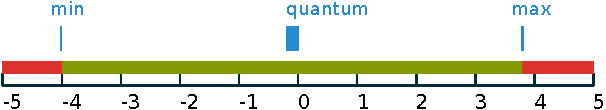
\includegraphics[width=\textwidth]{./src/img/fixedPoint.pdf}
\end{figureGraphics}

The test suite computes some values within the green(valid) area and the
red(invalid) area and performs the checks illustrated on figure \ref{fig:fixedPointTest} below.

\begin{figureGraphics}{Fixed point test suite}{fig:fixedPointTest}
    \includegraphics[height=0.6\textheight]{./src/img/fixedPointProcess.pdf}
\end{figureGraphics}

Below is a small description of the tests:
\begin{description}
    \item[Bound check] The \gls{pfw} should throw an error if we
        attempt to set an out-of-bound value.
    \item[Sanity check] If we manage to set the value, The \gls{pfw} should not modify too much
        the value. It can change by half a quantum at maximum.
    \item[Consistency check] The \gls{pfw} should accept the value it sent previously.
    \item[Bijectivity check] The \gls{pfw} should return the same value we provided it at the Consistency check.
\end{description}

\subsubsection{Rework the internal mechanism}
It was time to rework the internal
mechanism of the \gls{pfw}.

The \gls{pfw} can export parameters to a file. Fixed
point parameters can be exported as well.
\begin{itemize}
    \item When exporting them, the \gls{pfw} converts the value from
        its internal representation towards a floating point number, because that is
        easier to read.
    \item By converting that number, it also computes the amount of digits
        to use for display, or writing towards a file. This can result in
        \emph{rounding issues}, due to limitation of the \lstinline{setPrecision} \gls{cpp} method.
        TODO detail what were the issues (rounding to upper value, etc)
\end{itemize}
The fix I proposed was to replace the computation of displayable digits by something
easier, which is the \emph{Fractional part} of the fixed point number.

The example in listing \ref {lst:fixedPointProblem} illustrates a bound error check, and the output in the corrected version.

\begin{code}[language=bash, caption=$Q.2.3$ rounding issue example, label=lst:fixedPointProblem]
#  broken version  #
####################
$ pfw setParameter /Example/fixedPoint/q2.3 3.875
# Done
$ pfw getParameter /Example/fixedPoint/q2.3
# 3.9 <= this is not expected, since 3.875 is encodable!
$ pfw setParameter /Example/fixedPoint/q2.3 3.9
# Value 3.9 standing out of admitted real range
# [-4, 3.875] for FixedPointParameter /Test/test/q2.3
# ^ this is even weirder

#  fixed version  #
###################
$ pfw setParameter /Example/fixedPoint/q2.3 3.875
# Done
$ pfw getParameter /Example/fixedPoint/q2.3
# 3.875
\end{code}


% {{{2
\subsection{Multiple modem support}
With the \emph{bring your own device} trends, more and more smartphones support dual simcards. This case
is useful to use the same device for corporate and private purposes.
Besided, in some developing countries phone carriers do not cover the whole country. The habitants of those
countries need several phone carriers to use their smartphone smoothly.
For those purposes, the platform must support two modems.
Within the Intel Audio \gls{hal}, we are handling some voice processing algorithms from the signal coming from the modem.
Naturally, we have a \gls{pfw} plugin to abstract the modem. This plugin did not support multiple modems.

I had to add \emph{modem instance awareness} to the plugin. With the current implementation, it
is possible to have multiple Structure files, each describing a modem. This would theoretically allow
to support as many modems as we want.

TODO explain a bit more.

% {{{1
\section{Open-sourcing on GitHub}
In order to stimulate the usage of the \gls{pfw} for other projects than the Intel Audio \gls{hal},
our team decided to release the source-code on \gls{GitHub}.
This should favor external contributions via \gls{pullrequests} and motivate
the community to use the \gls{pfw}.

Around this activity, I covered several topics:
\begin{description}
    \item[Communicating, Documentating] the \gls{pfw} components.
    \item[Push, clean, enchance] the code to make sure no proprietary
        elements are made public.
\end{description}

% {{{2
\subsection{Parameter-framework newcomer's documentation}\label{sec:tutorials}

At the start of my internship, I had to inspect the \gls{pfw}'s
source code without any documentation. The idea was to have a fresh look at
this piece of software to determine if it was open-source ready, straightforward
to use, for someone who is unfamiliar with it.

While doing that, I struggled a bit with the basic usage of the framework. The
team decided that it would be nice to have some newcomer tutorials and examples,
for an easier adoption of the open-source community. So I wrote several
tutorials:
\begin{description}
    \item[Compile and install]
        is a step-by-step guide about how to get the \gls{pfw}'s sources,
        build it and install it as a standalone on Ubuntu.
    \item[Run a simple example]
        is a how-to about running the \gls{pfw} command-line interface,
        such as \lstinline{remote-process} and \lstinline {test-platform}.  In
        this how-to, the configuration and setting files are provided so that
        the user can focus on the results. The example covers music play-list
        changing based on a user's mood.
    \item[An introduction to the .pfw language]\label{desc:pfw-language}
        is a tutorial about the .pfw language. This language was
        created to simplify the writing of settings files for the
        \gls{pfw}. Those files are then converted into \gls{xml}, which is
        the only language the \gls{pfw} understands.
\end{description}
These tutorials have been written in \gls{markdown}, the standard format used
on \gls{GitHub}.

% {{{2
\subsection{Parameter-framework's intellectual property}
Intellectual property is very important at Intel. The \gls{pfw} is released under
BSD license. All the source files must contain the correct BSD license header according
to Intel's open-source policy.

\subsubsection{license checker}
Since there are 279 source files released currently on \gls{GitHub}, it seems a lot of
work to check all those files manually.
I wrote an internal tool in \gls{python} which performs the license check semi-automatically.
The script usage is quite straightforward and showed in listing \ref{code:license}.

\begin{code}[language=bash, caption=License checker usage, label=code:license]
usage: license_updater.py [-h] [--cpp | --mk] license root_location

Scans recursively trough directories to find source code which should be
updated with a new license header.

positional arguments:
    license        the license type: ['gpl', 'bsd', 'private']
    root_location  the directory to start scanning

optional arguments:
    -h, --help     show this help message and exit
    --cpp          (default) scan for C++ files: ('h', 'c', 'hpp', 'cpp')
    --mk           scan for Android make files: .mk
\end{code}


% {{{2
\subsection{Branch sync process}
Since we work internally on the \gls{pfw} and can receive external contributions via \gls{pullrequests},
it is quite difficult to keep both repositories in sync.
On figure \ref{fig:branch-process} we can see how we plan to synchronize the different code.

\begin{figureGraphics}{Final branch process}{fig:branch-process}
    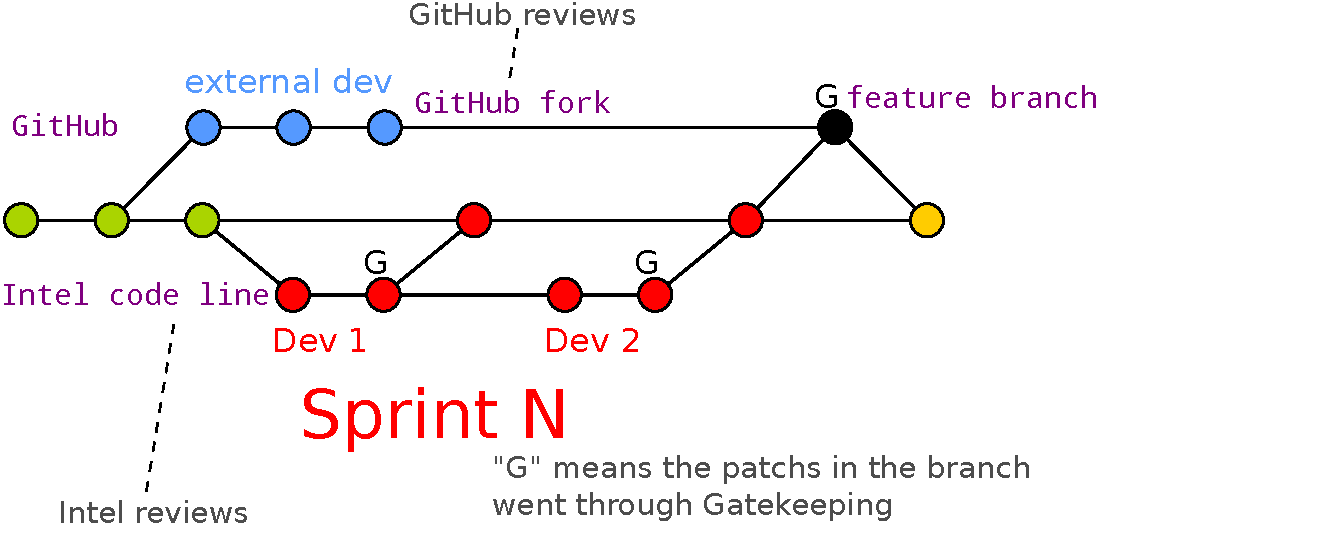
\includegraphics[width=\textwidth]{./src/img/branches-process.pdf}
\end{figureGraphics}


% {{{2
\subsection{Alsa plugin refactoring}
The Alsa plugin is used to handle \gls{alsa} (for desktop mostly) or TinyAlsa (for embedded \gls{android} devices mostly) subsystems.
For our internal uses, we patched some \gls{aosp} projects such as TinyAlsa which allows us to support proprietary controls.
The support of such controls was also implemented in the \gls{alsa} \gls{pfw} plugin. Since
we want to open-source the plugin, those proprietary features should be removed.

During the removal of those special controls, we also simplified the plugin
architecture by merging the controls and the mixer code. TODO removing templates.
The result is a far simpler design.
TODO detail.

% {{{2
\subsection{Code alignment}

When I had to update the different components on \gls{GitHub}, there were some issues:
Our internal version and the \gls{GitHub} one had diverged.
On figure \ref{fig:diverged}, we can see an overview of the branch state before I reworked them.

\begin{figureGraphics}{Repository divergence}{fig:diverged}
    \includegraphics[width=\textwidth]{./src/img/branch-divergence.pdf}
\end{figureGraphics}
Since all the components I uploaded on \gls{GitHub} had modifications which weren't present
in the internal source tree, I encountered the divergence issue for each project I
synchronized with \gls{GitHub} (Core, Alsa and Filesystem).

This was a very good exercise to improve my \gls{git} skill.

\subsection{Core upload}
The \gls{pfw} core is quite a big project, with about 30 000 lines of code.
Align the internal tree and the \gls{GitHub} version of this project required quite some work.
Some extra requirements apply on open-source projects, such as being compilable in a vanilla \gls{aosp} environment.

There is a \gls{GitHub} organization which groups all Intel open-source projects. This
organization is called \emph{01org}. I joined it during my internship in order to have admin rights
on the projects I had to open-source.

The \gls{pfw} core is available on \gls{GitHub}\footnote{\url{https://github.com/01org/parameter-framework}}

% {{{2
\subsection{Filesystem plugin upload}

The file system plugin is used for global access to the filesystem. This can be to
use \emph{/proc} entries for instance. I used this plugin as example in the rookie
documentation I wrote as described in section \ref{sec:tutorials}.

I also worked on an other example: \emph{controlling LEDS} via the filesystem
plugin on a Raspberry Pi.  This example was easy enough to be integrated into
the online documentation of the filesystem plugin, on \gls{GitHub}.

The filesystem plugin is available on \gls{GitHub}\footnote{\url{https://github.com/01org/parameter-framework-plugins-filesystem/}}

% {{{2
\subsection{Alsa plugin upload}

The \gls{alsa} \gls{pfw} plugin is used on within the Intel Audio \gls{hal}. It can also by used
on a linux desktop environement to handle \gls{alsa} mixers.

To demonstrate the power of this plugin, I wrote the README file which is on the
front page on this \gls{GitHub} project.  The README contains :
\begin{itemize}
    \item Build and install instructions
    \item Prerequisites for using this plugin
    \item A tutorial which details how to write the \gls{xml} files for this
    plugin in order to be able to change the master volume on a linux desktop.
\end{itemize}
I also reorganised some code within this plugin since we used to rely on proprietary \gls{aosp} modifications.
This plugin is now vanilla \gls{aosp} compatible, and can be used if the \gls{pfw} is installed.

The \gls{alsa} plugin is available on \gls{GitHub}\footnote{\url{https://github.com/01org/parameter-framework-plugins-alsa/}}
